\documentclass{article}
\usepackage[utf8]{inputenc}

\usepackage{graphicx}
\usepackage{color}
\usepackage{transparent}
\usepackage[export]{adjustbox}[2011/08/13]
\usepackage{tabularx}
%\usepackage{import}
\graphicspath{{fig/}}
%\graphicspath{{F:/Documents/fyp/doc/report/fig/}}
\usepackage{array}

\usepackage[ %backend=biber
    style=numeric,
    sorting=none]{biblatex}
%\bibliography{report.bib}

\nocite{*}
\addbibresource{report.bib}



\PassOptionsToPackage{hyphens}{url}\usepackage{hyperref}
\begin{document}
\begin{titlepage}
	\centering
	{\scshape\LARGE Sussex University \par}
	\vspace{1cm}
	{\scshape\Large Final year project\par}
	\vspace{1.5cm}
	{\huge\bfseries Scalable Distributed Computing using Hashing with Asynchronous I/O\par}
	\vspace{2cm}
	{\Large\scshape Michael Sledge\par}
	{\Large CN:121677\par}
	\vspace{1cm}
	{\Large Computer Science MComp\par}
	{\Large\itshape Department of Informatics\par}
	\vspace{1cm}
	{Supervised by}\par
	{\large George Parisis}

	\vfill

% Bottom of the page
	{\large 2016\par}
\end{titlepage}

\section*{Statement of Originality}
This report is submitted as part requirement for the degree of Computer Science at the University of Sussex. It is the product of my own labour except where indicated in the text. The report may be freely copied and distributed provided the source is acknowledged.
\begin{table}[b]
\centering
\bgroup
\def\arraystretch{2.5}
\begin{tabularx}{0.8\textwidth}{|l c l|X|}
\hline
& Signature & & \\\hline
\end{tabularx}
\egroup
\end{table}

\newpage

\section*{Summary}


\newpage
\tableofcontents
\newpage


\section{Introduction}

%this should give the motivation for the project. The aims of the project should at least be stated in the first paragraph, but preferably in the first sentence.
This project aims to create a system which enables the building of distributed computing applications, based on distributed hash table (DHT) lookup and routing.
%this sentence is awful
By implementing a consistent means of organising computing nodes and enabling communication between them without each node's applications needing knowledge of the other nodes in the system.
The system will be scalable and allow a large number of nodes to communicate efficiently.


% explain the structure of the report.
This report will cover professional and ethical considerations; related research and existing similar distributed systems, as well as asynchronous I/O implementations; more detailed technical requirements; details of the design and implementation of the system; and evaluation of its functionality and performance.


\subsection{Professional Considerations}
The BCS Code of Conduct \cite{bcscoc} sets out the following standards which may be relevant to this project: 2 c) “develop your professional knowledge, skills and competence on a continuing basis, maintaining awareness of technological developments, procedures, and standards that are relevant to your field.” and 2 d) “ensure that you have the knowledge and understanding of Legislation* and that you comply with such Legislation, in carrying out your professional responsibilities.”

From ‘Professional Competence and Integrity’ in Annex A Interpretation of the BCS Code of Conduct \cite{bcscoca}: “You should seek out and observe good practice exemplified by rules, standards, conventions or protocols that are relevant in your area of specialism.”

Existing libraries may be used in this project and their licenses must be followed, standards and conventions in languages used should be followed also.



%\section{REPORT BODY}

\section{Background Reading/Existing solutions}
\subsection{Distributed and DHT based systems}

\paragraph{Distributed Hash Tables}

\paragraph{The chord protocol} \cite{chord} uses consistent hashing to assign keys to nodes. It defines a set of functions which nodes use to build and maintain a chord network. Chord nodes in a network form a virtual ring in which each node is aware of its immediately adjacent nodes as well as several succeeding nodes.
Nodes are mapped into the same keyspace used for identifiers for the application.
Each node knows how to find the node that an identifier maps to, illustrated in fig 1. If the id is between the current node and its successor then it maps to the successor, otherwise it asks the furthest node it knows about that is not past the id in the keyspace. The succeeding nodes that a node has knowledge of are stored in a 'finger' table (illustrated as dashed arrows in figure \ref{fig:chord_succ}.) These are not necessary for functionality but they reduce the number of steps when mapping a key to a node.

\begin{figure}
\centering
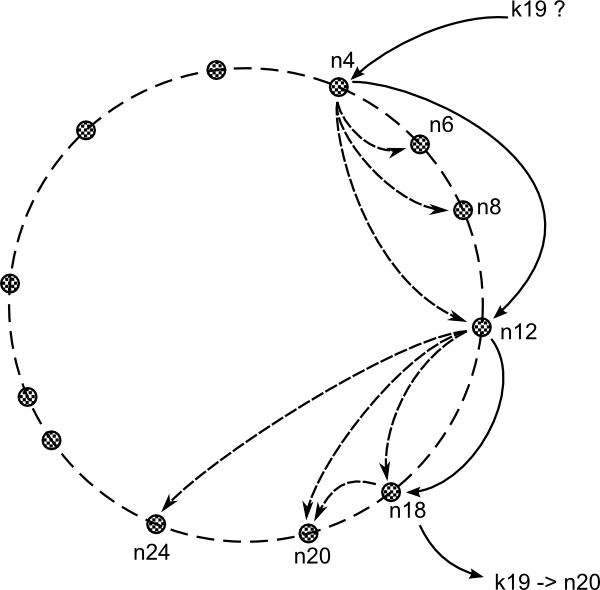
\includegraphics{chord_find-successor.png}
\caption{Finding the successor for key 19. Dashed arrows show which nodes a node has knowledge of (some have been omitted for clarity).}
\label{fig:chord_succ}
\end{figure}

The stabilisation that chord nodes run periodically is important to keep the network functional as the availability of nodes changes. Stabilisation is executed as follows: the node checks if there is a node between itself and its recorded successor, if there is it updates its recorded successor; then the node notifies its recorded successor of its existence so it can update its predecessor record if necessary. Nodes also periodically update their finger tables, and check whether their predecessor is still accessible.
Figure \ref{fig:chord_join_stab} shows the stabilisation process after a new node has joined the network.
\begin{figure}
\centering
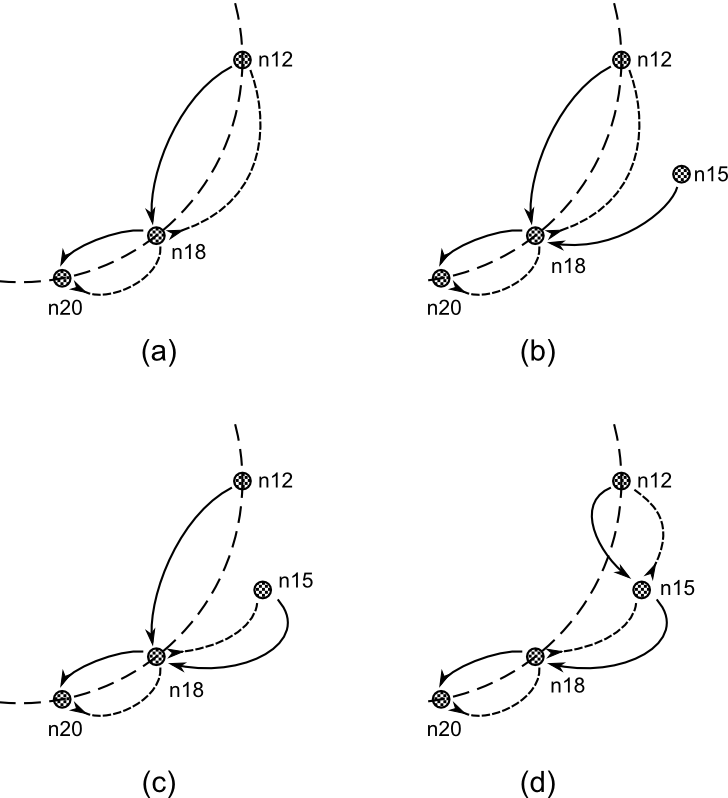
\includegraphics{chord_joining.png}
\caption{Node joining and stabilisation. (a) A chord network in a stable state. (b) new node n15 joins having found its successor (c) n15 runs its stabilisation and now n18 is aware of n15. (d) n12 runs its stabilisation and the network is back to as stable state}
\label{fig:chord_join_stab}
\end{figure}

There is an more extensive discussion of the chord protocol, along with my specific implementation in the design section.
\\
\\
\paragraph{Pastry} \cite{pastry}


\paragraph{Memcached} \cite{memcached} is a distributed in-memory caching system based on a distributed hash table intended for use in speeding up web applications by caching database entries, though it is possible to use it for other similar purposes. It is used by many large web companies.

Memcached uses spare memory on web servers to create a distributed in-memory cache which can be used to alleviate server load. This provides several benefits when compared to having each server managing it's own individual cache: the combined cache is much larger than individual caches; cached data is consistent any server requesting the a key in the cache will get the same value, whereas separate caches may not update data at the same time; improved scalability, as more servers are added to handle increasing load the size of the cache increases, making large scaling much easier than it would be with individual caches per server.
\\
\\
% pastry, tapestry, bamboo etc.


\paragraph{Mace} \cite{mace} is a toolkit for building distributed systems which “seeks to transform the way distributed systems are built by providing designers with a simple method for writing complex but correct and efficient implementations of distributed systems.” \cite{mace_quote} It is designed to provide a common 'language' to design distributed systems without having to implement the entire system from scratch, it provides and uses libraries to build systems. The restrictions mace imposes in this way allow for better options for debugging a distributed system.

Mace consists of it's own domain-specific C++ language extension to allow users to implement node functionality, a set of libraries which implement the functionality necessary to create and maintain distributed systems as well as common features for such systems. This allows its users to concentrate on the system being distributed and spend less time on the implementation of the distribution itself.

Nodes in mace are made up of one or more layers and each layer is built on an event driven state machine. Like Chord, Mace creates a virtual overlay network in which each node keeps a record of adjacent nodes, periodically updating these records and notifying the application when changes occur.
\\
\\

\subsection{Asyncronous I/O}

\paragraph{Libevent} \cite{libevent} is a cross platform C library which provides a single API for implementing event driven network servers using one of a number of mechanisms systems provide for event notification, to allow for asynchronous I/O operations. Libevent checks for events and runs the callbacks specified for each event in the queue. An event can be a notification for a socket becoming read- or write-able, a new connection on a listen socket or a timer event among other things. Libevent also provides bufferevents to simplify the task of using read and write buffers with socket events. Libevent also includes a simple HTTP, DNS and RPC (remote procedure call) implementations.

Libevent provides a single API for event notification which can use a range of underlying mechanisms provided by different operating systems (currently /dev/poll, kqueue(2), event ports, POSIX select(2), Windows select(), poll(2), and epoll(4)).

Libevent is used in a range of widely used applications, systems and tools, including Memcached, the Chromium web browser, and the Transmission Bittorrent client, among many others.
\\
%using libevent
Using Libevent involves setting up an \texttt{event\_base}, adding one or more events to it and running the event loop. Events can be setup to be triggered by a number of conditions: a file descriptor being ready to read from and/or write to; a timeout expiration; a signal occurring; or manual triggering. Internally Libevent's event loop checks for triggered events and marks them active, then runs the user set callbacks for all active events which have the highest priority and then moves to the next iteration.
Also provided are buffer events which use internal callbacks to read from the events file descriptor into a buffer and write from another buffer to the file descriptor when the file descriptor is ready and then call user set callbacks when the buffers are above or below user set watermarks.
\\
\\

\paragraph{Boost.Asio} \cite{basio} is a cross platform C++ library, similar to libevent, providing a consistent API for network and low level I/O programming with an asynchronous model. Its scope is slightly narrower than libevent's, so it doesn't include the simple protocol implementations.




\section{Requirements Analysis}
Build a high performance library for building DHT based systems with asynchronous I/O for scalability. Nodes should be independent and self organising, requiring no central authority, and be tolerant of joining, leaving and failing of nodes in the system.

\subsection{Functional requirements}
\begin{itemize}
\item
Creating and joining a network
\item
Finding the node a key maps to from any node on the network.
The algorithm finds the node a key maps to directly or finds the next hop and passes the job of finding it on to that node.
\item
Periodic stabilisation to account for change in availability of nodes.
Periodic checking for failures of adjacent nodes and arrival of new nodes. New nodes must notify at least one node of their presence.
\item
Allow sending of messages or data to other nodes for the application.
Once the node a key maps to has been found allow data to be sent to that node.
\item
Provide callbacks for the application when a message is received.
Allow the application programmer to provide functions which are called when specific events occur.
\item
Provide callbacks for notifying the application of changes in the availability of nodes that may affect it, i.e. the next and previous nodes. Specifically when the set of keys a node is responsible for changes.
\end{itemize}


\subsection{Non-functional requirements}
\begin{itemize}
\item
Provide high performance network communication between nodes
\item
Be highly scalable both in terms of number of nodes and the load of individual nodes assuming the application is able to handle such loads.
\item
Ease of use.
\end{itemize}

\section{Design and Building}

\subsection{Design Process}

The design involves multiple modules or layers
required considering both the internal functionality and the interface provided to users of the finished library.

\subsection{Design Principals}
Several design principals were employed to help reduce the chance of unhandled errors occurring and to simplify the task of building a complicated system.

\subparagraph{No global state}
This makes it easier to create thread-safe code and allow multiple instances to be instantiated within a single process. It allows for a more functional approach wherein all state has to be passed to functions as a arguments, this will mean that they can be implemented so to, as far as possible, always behave consistently way when given the same input.

\subparagraph{Layered structure}
The code will be organised into separate layers which utilise the layers below them but do not assume knowledge of layers above. this minimises interdependencies between modules.
This allows easier management of the project and means each component can be understood on its own, thus simplifying the task of building them.

\subparagraph{Defensive programming}
Errors in software are inevitable, however they can be reduced and managed with some thought. For example by checking all function input and checking function return codes to catch errors before they cause further problems, allowing

\subsection{Design Details}

\paragraph{Overlay network}
To facilitate the self-organisation of nodes and communication between them, a virtual 'overlay' network is created. It's design is based on the Chord protocol as referenced earlier. Each node on the network is assigned an identifier in the form of a hash of a user supplied parameter or 'name'. The overlay network itself takes the form af a virtual ring of nodes ordered by their identifiers, in which each node is aware the real location (i.e. IP address and port number) of and can communicate with one or more nodes with identifiers proceeding it's own. Figure \ref{fig:rtovmap} shows how nodes in a real network map into the virtual network.
\\
To maintain the network, each node is aware of several other nodes, specifically their immediate successor and predecessor, as well as several nodes in the finger table for improved lookup performance.

\subparagraph{Routing} The main functionality of the network is mapping identifiers to nodes, because at minimum each node knows about its immediate successor, this is be achieved by checking if the ID is between that of the current node and that of its successor, if it is then the ID maps to the successor, otherwise the successor is asked to find the node which the ID maps to. 
This works correctly, however in the worst case it requires querying every node in the system in turn to find the mapping. 
An improvement to this system is for each node to keep a cache of several nodes succeeding it, this is called the \textit{finger table} and consists of a list of nodes after the current at progressively larger intervals.
Specifically it contains \textit{m} entries where \textit{m} is the number of bits in identifiers. Entry \textit{k} refers to the node that is the successor of $(n + 2^k) mod 2^m$ where \textit{n} is the identifier of the current node.
The \textit{finger table} is used for mapping by asking the last node in the finger table with an ID lower than the one being mapped rather than just the successor.
Figure \ref{fig:fingersRbttr} shows the improvement using a finger table can make for lookup.

\begin{figure}
\centering
\def\svgwidth{\columnwidth}
\input{./fig/nodes_to_overlay_map.pdf_tex}
\caption{Mapping of nodes on a real network (e.g. the internet) to a virtual overlay network. Each node is aware of at least the next node in the ring}
\label{fig:rtovmap}
\end{figure}


\begin{figure}
\centering
\def\svgwidth{\columnwidth}
\input{./fig/finger_table_improvement.pdf_tex}
\caption{Use of a finger table improves lookup performance by reducing the number of hops to find the node an ID maps to.}
\label{fig:fingersRbttr}
\end{figure}


\subparagraph{Stabilisation} There are several things which need to be done in order to maintain the network as nodes may join or leave at any time. The first stage is to check the availability of the nodes successor as this is the main point of contact with the network, for this reason each node keeps a list of several successor nodes for use in the event that the immediate successor becomes unavailable.
\\
The stabilisation process consists of several stages, firstly a node checks that the successor nodes are available and removes any which aren't.
Next the node verifies it is in the right place on the network by asking it's recorded successor for it's predecessor. This will either be itself, a new node that has joined the system or none in the case that it's original immediate successor has become unavailable. The node is now aware of its successor, either it hasn't changed or it has the been given a new one. The next step is to 'notify' the successor so that it is aware of its predecessor for use in future stabilisations.
Nodes also periodically check the availability of their predecessors.
\\
The last stage is updating the finger table, which is simply a matter of asking the successor to find the successor of several pre-determined identifiers as defined in the routing description.



\paragraph{The Network layer}
The network layer handles open connections as well as the listen socket. It mostly acts as a wrapper for libevent and provides a simplified interface for the layers above. The main data structure is \texttt{struct net\_server} which is an instance of the net layer which needs to be passed to the majority of functions. It holds references to an event base (libevent's main data structure); open connections; and the listen socket. The layer contains functions for creating, activating and configuring connections.

\subparagraph{Usage}
Initialise a new server instance by providing a listen port number and a callback function and argument for accepting incoming connections. Once any other setup is complete, the function \texttt{net\_server\_run} can be called which starts the event loop and does not return until the loop exits and as such users must start another thread if they wish for their application to do more than wait for incoming connections.
\\
On receiving notification of an accepted connection (via callback), the application should set read, error/disconnect, and optionally write handlers for the newly accepted connection.
\\
Users can create outgoing connections by providing a remote IP and port this sets up the connection internally but does not activate it, this allows the user to add data to the write buffer before connecting if desired.
\\
Both accepted incoming and outgoing connections use the same interface, allowing setting of callback functions for read, write and other events; setting of the callbacks' custom argument; getting the connection's read and write buffers; setting the connection's timeouts; getting the remote address (useful for some types of messages on incoming connections); and getting the underlying buffer event for finer control

\subparagraph{Internals}
The net server keeps a list of references to open connections and keeps track of the callbacks that have been set for each one. It also has a mutex lock for the connection list to prevent concurrent modification as it is likely that the event loop thread may accept a connection while another thread requests creation of an outgoing connection.
\\
Connections use libevent's \texttt{buffer\_event} which can be used to automatically read incoming data from a socket to a buffer and write data to a socket from a buffer as the socket becomes readable and writeable respectively, they can be set to invoke there callbacks when the buffers contain more or less than a given amount of data.
\\
Most of the network layer's functionality is that for interacting with connections

\paragraph{The Node layer}
The node layer is the main body and contains code for creating, joining and maintaining the overlay network  and routing, these are together due to the fact that joining and maintaining the network requires routing messages between nodes. Much like the net layer its main data type is a handle to a node instance, the interface similarly consists of a function to initialise a new node instance and functions to join an existing network or create a new one. 

% details on overlay network, finger table etc. go here somewhere

\subparagraph{Usage}
% put all functions which should be usable by the app here
Users of this library will setup a node by calling \texttt{node\_create}, then setting up callbacks for incoming messages and join and leave notifications if necessary.
\\
Then the user can call \texttt{node\_network\_join} with the address of an existing node to join an existing network or \texttt{node\_network\_create} to create a new network. Both functions will call a given callback when he network has been joined or created respectively.

\subparagraph{Internals}
A node instance contains a reference to its own net server instance.
The node layer can be split into a few sub modules: Handling incoming messages from other nodes; network maintenance; message routing; initiating communications with other nodes
\\
Routing: the most important functions are \texttt{node\_find\_successor} and \\\texttt{node\_find\_successor\_remote} as they are used directly and indirectly by most other functions. These functions map IDs to nodes by checking if the current node or it's successor is the successor of the given ID and if not asking another node the same thing until the successor is found.
\\
Stabilisation and network maintenance: There are three groups of functions which are run periodically, they are: stabilise, which involves ordering nodes correctly in the overlay network; fix fingers, which ensures the node's finger table is up to date; and periodic checks of the availability of neighbouring nodes.
% this is poorly worded
The stabilise function updates the node's successor if necessary, by asking the node currently recorded as the successor for it's predecessor, and then notifies the updated successor that the current node is it's predecessor.
The fix fingers function iterates through the positions in the finger table and finds the relevant node, again using \texttt{node\_find\_successor}, and updates the table.
Periodically The availability of the node's predecessor is checked by sending it a message.
\\
Incoming handling: When the network layer notifies the node layer that an incoming connection, the node layer sets up the callbacks for the connection. Once the header of the incoming message has been received, the type and content length are read and the relevant callbacks for each type of message are setup or called immediately if the content is already all in the connection's read buffer. There are functions for handling each type of incoming message.
\\
Utility functions: There are several utility functions used by several other functions which simplify their own code.
%net interface
\texttt{node\_send\_message} takes a \texttt{struct node\_msg} formats it and writes it to an open connection, the similarly named \texttt{node\_connect\_and\_send\_message} opens a new connection to the specified node and calls \texttt{node\_send\_message} with it.
%hash id helpers
\texttt{node\_id\_compare} takes two identifier hashes and returns 1, 0, or -1 to indicate that the first is greater than, equal to, or less than the second respectively.
\texttt{node\_id\_in\_range} takes three ids identifier hashes and returns 'true' if the first falls between the second and third in the identifier space.
The \texttt{get\_id} function takes a string and maps it to an identifier hash

\paragraph{ID hashes}
The hashing function chosen for the identifier space is SHA-1. SHA-1 provides 160 bit hashes which is a relatively small space compared to other cryptographic hash functions and has a higher probability of collisions. This however, is not a cause for concern as collisions would only have an effect on the system if two nodes were to have the same ID, which due to the relatively low number of nodes is highly unlikely.
% Do I need to cite this? probably I guess
The library uses the OpenSSL \cite{openssl} SHA-1 implementation.

\paragraph{Communication Protocol}
Messages sent between nodes use a TLV (type-length-value) format, in other words they consist of a header, containing a single byte indicating the type of message and a 4 byte value indicating the length of the body, and the body itself which contains the actual information formatted according to the message type.

\subsection{Using the Library}

Most interaction with the library is with the node layer, though some interaction with the net layer is necessary.
The first stage is initialising a node with a listen port and a unique name used for the nodes identifier by calling \texttt{node\_create}. This allocates all necessary data structures and sets up the network layer.
Next calling \texttt{node\_network\_create} or \texttt{node\_network\_join} providing a callback for when the network has been successfully joined and, in the latter case, the address of an existing node in the network.
This starts the event loop and as such does not return until the node is shut down, This is why the callback is necessary, the application should utilise it to start one or more threads for its functionality.
When a node receives a message for the application, a users specified callback is called with the message, the application should use this to pass the relevant information to its processing thread(s) to prevent blocking of other network activity.
Figure \ref{fig:startlib} shows an overview of the process of setting up and running a node, and figure \ref{fig:runlib} shows the main interactions that an application will have with the library as well as the major internal interactions

\begin{figure}
\centering
\def\svgwidth{\columnwidth}
\input{./fig/start_lib.pdf_tex}
\caption{Process of setting up a node with the library, first call setup with a name and listen port number, then join or create a network, once this is done a given callback is called to allow the node to start its own functionality which should be run in separate threads.}
\label{fig:startlib}
\end{figure}


\begin{figure}
\centering
\def\svgwidth{1.4\columnwidth}
\begin{scriptsize}
\makebox[\columnwidth][c]{\input{./fig/run_lib_curr.pdf_tex}}
\end{scriptsize}
%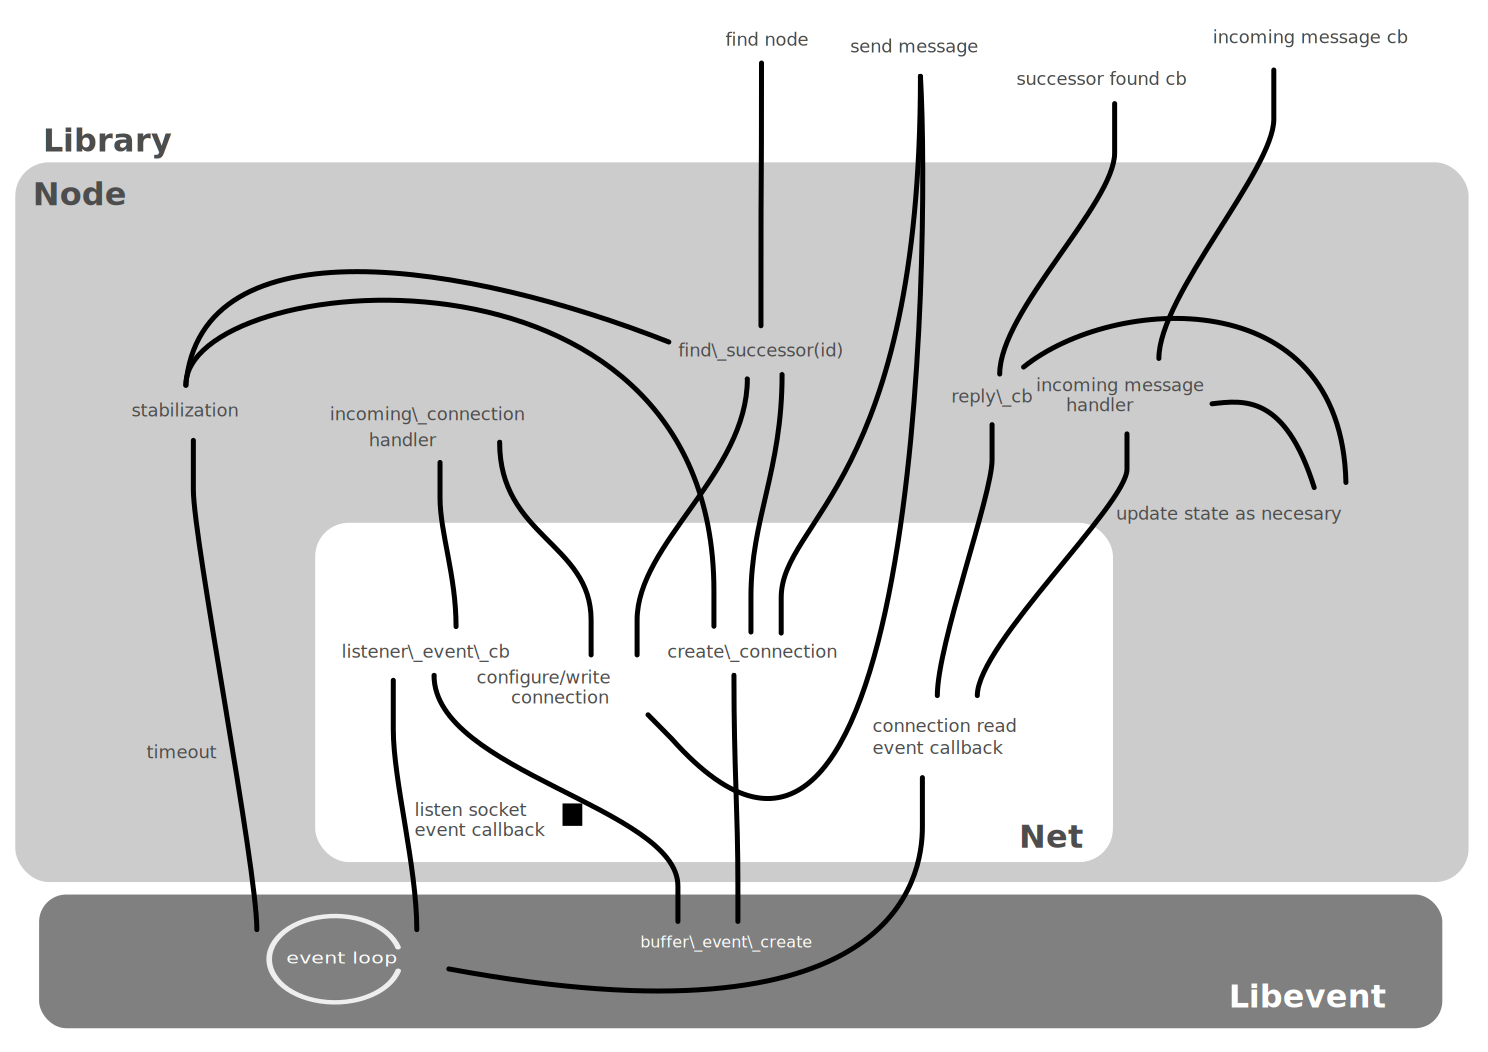
\includegraphics[width=1.6\textwidth,center]{run_lib_curr.png}%
\caption{Main interactions with and within the library once running }
\label{fig:runlib}
\end{figure}

\subsection{Example applications}

\paragraph{1. textsend}

This is a simple command line application to demonstrate basic functionality. It will join an existing network if given the address of a node, or create a new one. Once in a network this application takes text input from \texttt{stdin} and sends it to the node it maps to. Upon receiving a message from a node it is printed to \texttt{stdout}
\\
\\
%pub/sub, storage, group communication etc implementation expectations

There are a few other applications which could be implemented as follows

\paragraph{2. Publish subscribe system} A publish-subscribe system allows data producers (publishers) send messages to receivers (subscribers) without either necessarily knowing about the existence of the other. Specifically publishers output data with a specific label or topic into some intermediary system which then forwards the data to subscribers to that topic.
To implement such a system using the library, the application would map topics to IDs using the topic name and then the successor node of that ID would be responsible for that topic. Nodes could subscribe to a topic by sending a \textit{subscribe} message to the node responsible for it, which would then add that node to its list of subscribers. Publishers would publish to topics in the same way, sending a \textit{publish} message to the node responsible for the topic, which then sends the message on to all registered subscribers to the topic.
% subscribe to topic
% publish to topic
% topic -> id => node n
% so node n is responsible for topic
% subscriber message n with 'subscribe'
% n keeps a list of subscribers to topics it is responsible for
% publishers send data for topic to n
% n sends data from publishers to all subscribers


\paragraph{3. Distributed storage}


\section{Testing}

Much of the code in this project is difficult to test because of the fact that much of it depends on network communication and having the system running, for that reason most testing was done by setting up a small network of nodes running a simple application.

\subsection{Simulated real world testing}

Once the minimal required functionality had been implemented, I was able to test the functionality using a simple application with minimal functionality.

\section{Evaluation}

Figure \ref{fig:fingerperf} shows the mean number of hops to find the successor of a given identifier

\begin{figure}
\begin{center}
\makebox[\columnwidth][c]{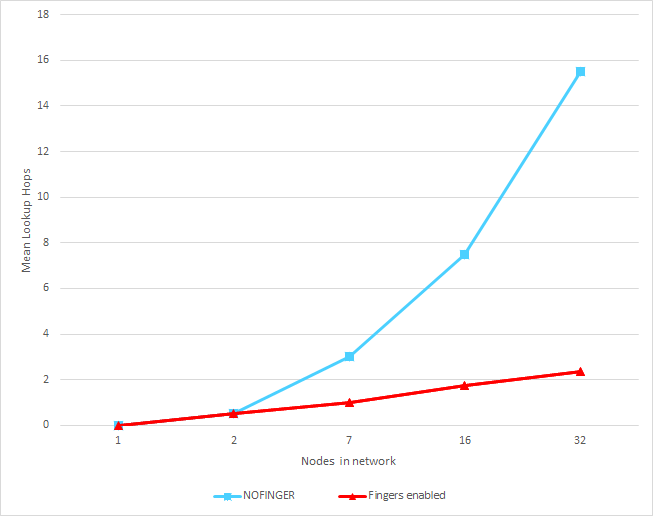
\includegraphics[width=1.2\columnwidth]{finger_performance.png}}
\end{center}
%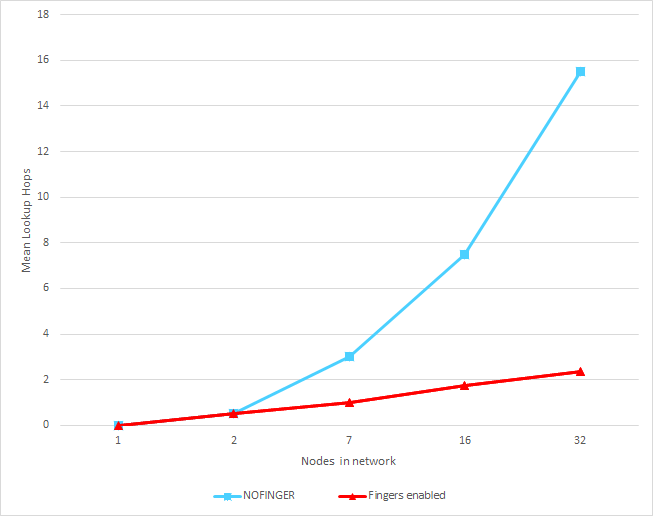
\includegraphics{finger_performance.png}
\caption{Graph showing average hops (nodes which need to be asked) to find the successor of an I.D.}
\label{fig:fingerperf}
\end{figure}



\section{Conclusion}

have succeeded in building a library for implementing distributed systems, which provides an interface for sending messages between nodes and handles organising and maintaining the network using asynchronous I/O for network communication.

Ease of use can be difficult to evaluate, however the \texttt{textsend} application gives an indication that the library provides an easy to use interface
% evaluation summary

\subsection{Future work}

There are several enhancements I would like to make beyond the current functionality, which could make real world usage more viable.
%  Configurability
\paragraph{Configurability and tuning} Allowing configuration and tuning of parameters such as the stabilisation interval could help improve performance and stability of the network, depending on the use case, for instance one system may expect the availability of nodes to remain fairly constant so heigh frequency stabilisation may be unnecessary, while another may expect a high rate of \textit{churn} (nodes joining and leaving frequently) and so would need much more frequent stabilisation.

%  Security
\paragraph{Security} I would like to implement SSL based connections between nodes to allow for secure communication and verification of message origin.
Additionally, allowing use of domain names for addressing nodes in addition to SSL would allow for implementation of a system which only allows specific nodes to join the system.

% network info
\paragraph{Network monitoring} Currently, there is no means of monitoring the state of the network as a whole, other than using the debugging info from each individual node. It should be relatively simple to add more types of message for gathering information about the network, for instance the number of nodes could be determined by a message sent around the entire ring from each node to its successor until it arrived at the node which originated the message.

\section{References}

%\bibliographystyle{unsrt}
%\bibliography{report}
\printbibliography


\section{Appendices}
\appendix
\section{Message protocol}

Messages are made up of a single bit defining the type of the message; a 4 byte value for the length of the message body; and the optional, variable length message body.

\subsection{Type bit values}
\begin{tabular}{|l | l|}
\hline
\texttt{'S'} & Ask node for successor of id \\\hline
\texttt{'s'} & Return successor of id \\\hline
\texttt{'P'} & Ask a node for its predecessor \\\hline
\texttt{'p'} & Returning a node's predecessor \\\hline
\texttt{'N'} & Notify another node that the sender believes it is that node's predecessor \\\hline
\texttt{'A'} & Used to check the availability of a node\\\hline
\texttt{'a'} & Reply to confirm that a node is operating \\\hline
\texttt{'M'} & The contents of the message is for the application using the library \\\hline
\texttt{'0'} & Signifies Unknown message type \\\hline
\end{tabular}

\subsection{Body Layouts}
\newcolumntype{L}{>{\arraybackslash}m{9cm}}
\begin{tabular}{|l | l | L|}
\hline
\texttt{'S'} & ID & The ID to find the successor of\\\hline
\texttt{'s'} & 'Y' ID IP port & the char 'Y' to indicate success followed by the i.d. i.p. and port of the node found\\\hline
\texttt{'P'} & N/A & no body necessary\\\hline
\texttt{'p'} & 'Y' ID IP port & the char 'Y' to indicate success followed by the i.d. i.p. and port of the node's predecessor \\\hline
\texttt{'N'} & ID port & the i.d. and listen port of the node dong the notifying (i.p. address obtained from connection) \\\hline
\texttt{'A'} & N/A & no body necessary\\\hline
\texttt{'a'} & Y & simple confirmation message\\\hline
\texttt{'M'} & N/A & Application dependant\\\hline
\end{tabular}






\end{document}
